\documentclass[a4paper, oneside]{book}
%Use package definitions
\usepackage[margin=1.4in]{geometry}
\usepackage[utf8]{inputenc}
%Serif font
\usepackage{cmbright}
\usepackage[T1]{fontenc}
\usepackage{textcomp}
\usepackage{amsmath, amssymb, bm}
\usepackage{pdfpages}
%Line through stuff
\usepackage{centernot}
\usepackage{transparent}
\usepackage{varwidth}
%Custom boxes
\usepackage[most]{tcolorbox}
\usepackage{xcolor}
\usepackage{url}
\usepackage{hyperref}
%Algorithm environments
\usepackage{algorithm}
\usepackage{algpseudocode}
%Header
\usepackage{titleps}

\newpagestyle{main}{
\setheadrule{.4pt}% Header rule
\sethead{MATH70027 Project 1 Solutions}{}{CID: 01859216}
% \setfootrule{.4pt}
\setfoot{}{\thepage}{}
}
\pagestyle{main}
%Space between paragraphs
\setlength{\parskip}{10pt}
%No indentation on the first word of a new paragraph
\setlength{\parindent}{0cm}
%Define where images are stored
\newcommand{\imgpath}{/home/isaac/Documents/Maths/Year_3/LaTeX/Images/}
%Creating a new color box
\newtcolorbox{blackbox}[1][]{colframe=black,colback=white,sharp corners,center,#1}
%Creating the title

%Creating the title
\title{MATH70027 - Scientific Computation Project 1 Solutions\author{CID: 01859216}\date{\today}}


% -----------------------------------------------------------------------
\begin{document}
\maketitle


\section*{Part 1}

\subsection*{Question 1.1}
Part1 uses a mixture of insertion sort and binary search to sort the input
list Xin in non-decreasing order.
It first sorts the first section of the list (up to and including the istar$^\text{th}$ index)
using insertion sort. Then the remaining unsorted right side of the list is sorted
using binary search. This works by finding the correct position/index in the sorted left side
for each element in the unsorted right side, using binary search, and then moving the element
to this position, bumping up the other elements to make room.

When it comes to computational complexity, we first consider the insertion sort part.
Clearly insertion sort is $O(n^2)$ in the worst case, i.e when the list is in reverse order,
since we will have 1 + 2 + 3 + ... + n - 1 comparisons = $n(n-1)/2$ i.e $O(n^2)$, where $n$ is
the length of the list. Of course in this case $n = \text{istar} + 1$ and therefore we have
$O(\text{istar}^2)$ worst-case and average-case time complexity for the first half ($O(\text{istar}^2)$ for best case), and O(N) memory complexity.
Then for the second part of the algorithm, i.e the binary search part, we have
N - (istar + 1) elements to find a home for amongst istar + 1 elements, using binary search.
So therefore we have $O(\log(\text{istar} + 1) * (N - \text{istar} + 1)) = O(N\log(\text{istar}) - \text{istar} * \log(\text{istar}))$ worst case time complexity for the binary search part.
Then we also have to insert into the list each time, which takes $O(N)$ for each iteration
and so we have $O(N^2)$ total worst-case cost of inserting into the list.

So overall we have $O((N - \text{istar})\log(\text{istar}) + \text{istar}^2 + N^2)$ worst-case time complexity and $O(N)$ memory complexity.
Of course istar is a function of $N$ and therefore our overall worst-case complexity if $O(N^2)$.
Using this we see that istar should be as small as possible.

\subsection*{Question 1.2}
So in order to investigate the trends in wall time as a function of $\text{istar}$ and $N$,
we fix either $\text{istar}$ or $N$ and then vary the other. For each combination of $N$ and $\text{istar}$
we run $\text{part1}$ with a randomized list of integers of length N and measure the wall time
that the function took to run.
We do this $\text{num\_runs}=10$ times for each combination of istar and N and then take the
average time, so as to dampen the effect of any anomalous results. Then
we plot the dependent variable on the y-axis (walltime in seconds) and the independent variable ($\text{istar}$ or $N$)
on the x-axis. (See Figure \ref{fig:plots} below for plots).

\begin{figure}[htpb]
    \centering
    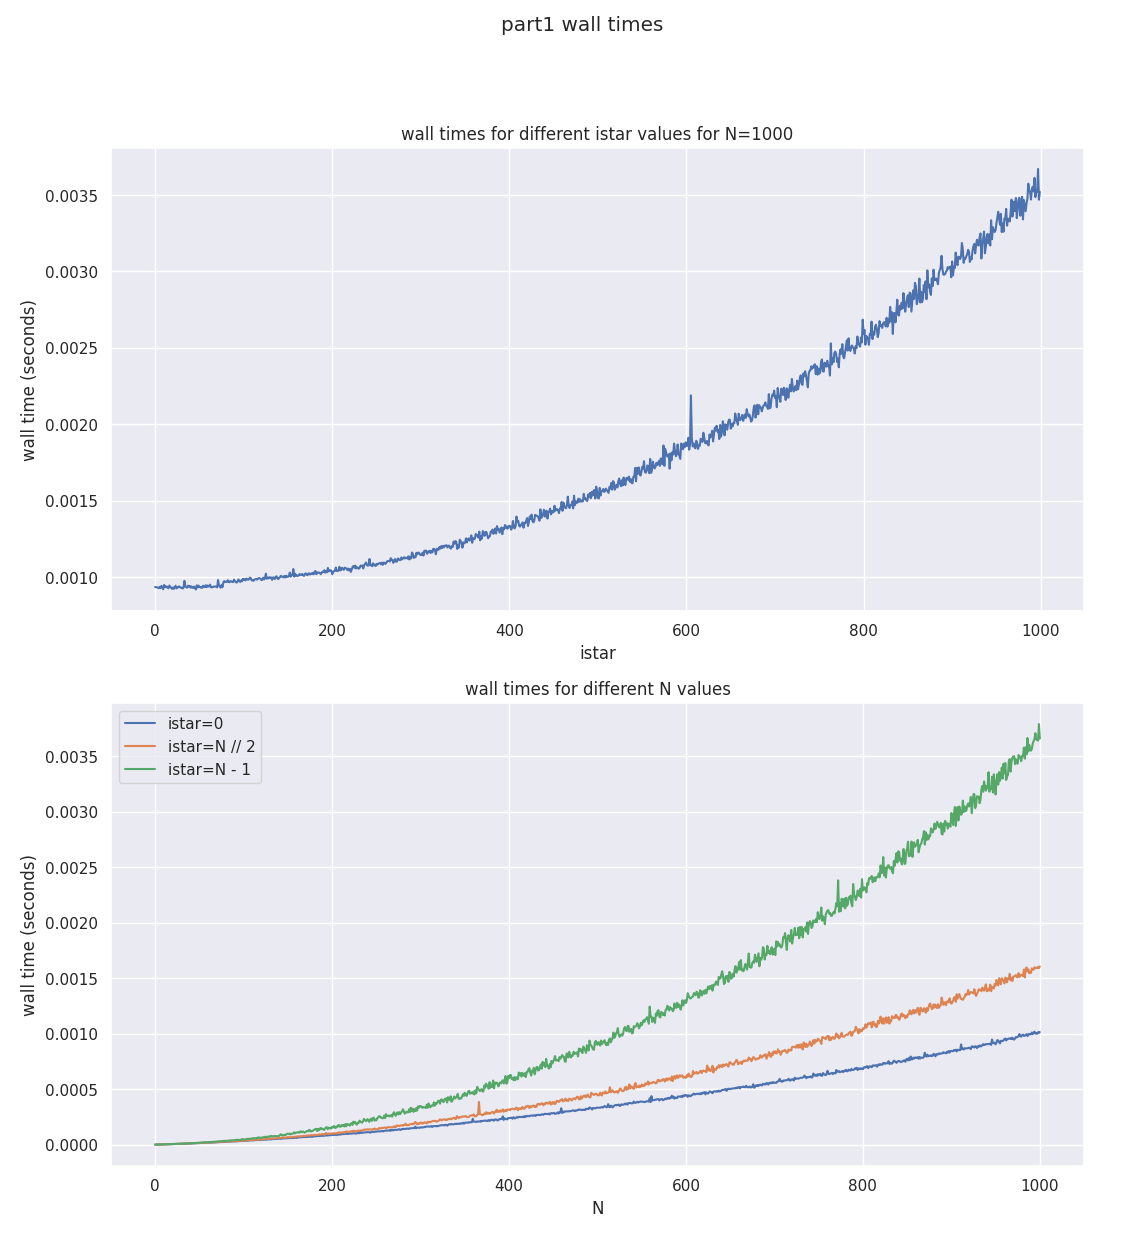
\includegraphics[origin=c,width=1.0\textwidth]{./images/sco_fig_1.png}
    \caption{Question 1.2 plots. Plotting wall time as a function of N and istar.}
    \label{fig:plots}
\end{figure}

In the first plot, we see that $\text{istar}$ is the independent variable and we have kept N fixed at 1000.
Our results indicate that wall time is a quadratic function of $\text{istar}$, i.e
with $N$ held fixed, part1 has time complexity $O(\text{istar}^2)$. This agrees exactly with our
theoretical time complexity result from question 1. Nice.

Then in our second plot we plot the wall time as a function of N, varying N from 0 to 1000.
We use three values of $\text{istar}$, as a function of $N$. $\text{istar} = 0, \text{istar} = N // 2$ and $\text{istar} = N - 1$.
The plot for $\text{istar}=0$ seems to have a very week quadratic relationship in $N$.
This agrees with our theoretical result, since $O((N - 0)\log(0) + 0^2 + N^2) = O(N^2).$
Then when $\text{istar} = N // 2$ we see what looks like stronger quadratic behaviour.
This also agrees with our theoretical result, since when $\text{istar} = N//2$ we have $O(N\log(N) + N^2)$ complexity.
Finally for $\text{istar} = N -1$ we observe strongest quadratic behaviour in $N$. This also agrees with our theoretical
result, since we have $O((N - \text{istar})\log(\text{istar}) + \text{istar}^2 + N^2) = O(\log(N - 1) + (N - 1)^2 + N^2)$.

\section*{Part 2}

\subsection*{Question 2.2}
We implement a multi-pattern version of Rabin-Karp.
First we find all \textbf{unique} contiguous subsequences/substrings of $T$ of length $m$.
(From now on we will refer to these simply as subsequences).
Then we pre-compute the hashes for all of the subsequences
and define a map which maps each unique hash to a list of the subsequence indices
of the subsequences with corresponding hash. This is perhaps best demonstrated with an example.
Suppose $T := \text{CATCATCATG}$ and  $m := 3$. Then the possible unique subsequences (preserving ordering)
are  $\text{CAT}, \text{ATC}, \text{TCA}, \text{ATG}$. We define $k$ to be the index 
of the subsequence in the list of unique (order preserved) subsequences of T.
E.g  
\begin{align*}
    \text{CAT} &\implies k = 0, \\
    \text{ATC} &\implies k = 1,\\
    \text{TCA} &\implies k = 2,\\
    \text{ATG} &\implies k = 3.
\end{align*}

Then suppose the hashes are as follows:
\begin{align*}
    h(\text{CAT}) &= 100, \\
    h(\text{ATC}) &= 120,\\
    h(\text{TCA}) &= 130,\\
    h(\text{ATG})&= 100.
\end{align*}
Then our map would be:
\[
    \{100: [0, 3], 120: [1], 130: [2]\}
.\]
It would of course be simpler to just map each hash to each index (without the lists),
but since we can have hash collisions, (as demonstrated in the above example), we need
to use lists.

We will refer to this map as our \textit{hashtable}.

Then we convert $S$ to base $4$, and define this to be $X$. We then loop over every
possible starting index and calculate the rolling hash, using the Rabin-Karp method
given in lectures. We then check if this hash exists in our hashtable, and
if it does, we plug in the hash into our hashtable and get out the list of possible
subsequence indices which correspond to the subsequences with matching hash.
We then loop over each possible index, recover the subsequence and then check for a string match.
(We do this to handle collisions). If we get a match, then we store this index.

We store these indices in a second map/dictionary, which maps the unique subsequences to
a list of their matched indices in $S$. For example, if we continue the above example
with  $S := \text{TACATGCAT}$ then this map will look like:
\[
    \{\text{CAT}: [2, 6], \text{ATC}: [], \text{TCA}: [], \text{ATG}: [3]\}
.\]
Then finally, since the question asks for all subsequences of $T$, not just the unique ones,
we apply our map to all of the m-length subsequences of $T$, to get $L$. E.g
\begin{align*}
    T &= \text{CATCATCATG}, \\
    \implies L &= [[2, 6], [], [], [2, 6], [], [], [2, 6], [3]]
\end{align*}

This solution is efficient for multiple reasons. Firstly we have the obvious benefits from
using Rabin-Karp rolling hashes over just string matching, reducing checking matches
to $O(1)$ from $O(m)$ for non-matches. So if we have a lot of near misses, this will
save a lot of time. Then also by precomputing the hashes and using a hashtable we also save a lot of time
because we don't have to loop over each subsequence and then search over all of S every time.
Also by only considering \textbf{unique} subsequences in $T$, and building a map
we also save a lot of time, meaning we don't have to waste time, re-checking matches
for duplicate subsequences of $T$. 

So in terms of complexity, firstly finding all unique subsequences of $T$ takes $O(l)$.
Then when generating the hash table, calculating each hash takes $O(m)$, and we do this
for every unique m-length subsequence in $T$. In the worst case we could have $l - m + 1$
unique subsequences and therefore building our hashtable will have $O((l - m + 1)m = O(lm - m^2)$
worst-case time complexity. Then converting $S$ to base 4 will take $O(n)$.
Then for the main loop, at each iteration we perform a hashtable lookup ($O(1)$)
then we loop over each possible $k$ and check if $S[i:i+m] == \text{subsequences}[k]$.
As long as we use a big enough prime number, it should be pretty rare to get collisions
in our subsequences hashes, so the majority of our possible k lists (values from our hashtable)
will have length 1. So we don't need to be concerned about looping over each possible $k$ in our complexity calculations.
Checking the string matches takes $O(m)$, so therefore our worst-case complexity for
the main loop is $O((n - m + 1)m) = O(nm - m^2)$.

Then finally applying our map to all the non-unique subsequences of $T$ takes $O(l - m)$.

So combining everything we have worst-case runtime complexity $O(nm + lm - m^2)$.

Note that the average complexity should be much better, especially when have a lot
of near misses. The average complexity will be closer to $O(n + lm - m^2)$.

Then in terms of memory complexity, we are storing a list of unique subsequences and two dictionaries,
all with length equal to the number of unique subsequences (assuming no hash collisions for subsequence hashes).
So clearly we have $O(l - m)$ worst case memory complexity.

% -----------------------------------------------------------------------
\end{document}
